
\documentclass[runningheads]{llncs}
\usepackage[section]{placeins}

\usepackage{hyperref}
\usepackage{graphicx}
\usepackage{booktabs}
\hypersetup{
    colorlinks=true,
    linkcolor=blue,
    filecolor=magenta,      
    urlcolor=cyan,
    pdftitle={Overleaf Example},
    pdfpagemode=FullScreen,
    }
\begin{document}

\title{COMP3330 Assignment1}
\author{Sebastian Hadley}
\institute{University Of Newcastle}
\maketitle

\begin{abstract}
In this report, we assess the effectiveness of different methods of solving Machine Learning problems by solving a selection of problems with different methods and judging how different factors can impact the performance of the solutions.
\end{abstract}
\section{Question 1}

The 2 spiral-problem is quite difficult as it is a relatively small dataset with complex relations that determine the way each data point is classified, because of this it is difficult to build a Neural Network complex enough to identify the correct decision boundaries while also not over-fitting to the training data.
 
\subsection{Part a}

 For the "original dataset" of Lang and Witbrock (1988), different feed-forward Neural Network architectures were experimented with, including varying the number of layers, neurons per layer,learning rate and activation functions. The performance was evaluated on  the different configurations using 10-fold cross validation with each fold being broken up into test and training sets to ensure ability to generalize was being assessed. The quantitative metrics that were judged were, loss and accuracy as well as a qualitative analysis of the decision boundaries. The decision boundaries were output for each fold, as well as a final decision boundary that took the mode class predicted for each point within the grid over all the decision boundaries to output an average decision boundary over the 10-folds.

In the initial attempt the model was constructed with 2 hidden layers each containing 8 neurons, that used the Relu activation function with the output layer using SoftMax. This model was initially tested with a learning rate of 0.01 over 100 epochs, with a few attempts at adjusting the hyper-parameters to tune the results, this architecture performed fairly poorly for all the different hyper parameters that were attempted. \hyperref[tab:1A2LayerResults]{Table~\ref*{tab:1A2LayerResults}} shows the results of a few attempted hyper parameters.

The most successful of these quantitatively is likely the 8 neuron, 100 epoch version, however the version that used 1000 epochs had a promising average decision boundary, that seemed to resemble a spiral however still had alot of jagged edges and holes in the spiral shapes. \hyperref[fig:FirstFFNNDecision]{Figure~\ref*{fig:FirstFFNNDecision}}


\FloatBarrier

These results indicated that despite the small dataset, the relationship between the points is complex enough that we would need to additional layers and neurons. After experimenting with different options, the most consistent results were achieved by a model containing 5 hidden layers with the first using Relu and the rest using the LeakyRelu activation function, with SoftMax in the output layer as well as the hyper parameters shown in this table. \hyperref[tab:1AFinalModelArchitecture]{Table~\ref*{tab:1AFinalModelArchitecture}}

This Model performed quite well on both the training and test sets, with accuracy being better then the loss, 1 of the 10 folds seemed to go astray leading to it  not accurately classifying the test sets however even those folds still outperformed the previous models discussed above.

\counterwithin{table}{chapter}
\begin{table}[ht]
  \centering
  \caption{Average Results of Final Model Architecture}
  \begin{tabular}{c c c c c}
    \toprule
     Training Loss \quad & Training Accuracy \quad & Test Loss \quad & Test Accuracy \quad & Time Taken\\
    \midrule
    0.11 & 0.95  & 1.06 & 0.84 & FILL IN LATER \\
    \bottomrule
  \end{tabular}
  \label{tab:1AFinalModelAverageResults}
\end{table}


These results are promising, however the time taken was significantly longer then the previous models, the speed is especially poor in relation to the size of the dataset however the relationships that determine which spiral a point fell into are complex which does make the time more acceptable.

The decision boundaries for this model also are very good showing a clear spiral shape on all but 1 of the folds, with the average looking particularly clean. This boundary shows that the model is successfully able to learn the shape of the data consistently over 10 folds, which is even better considering that the model is also successful in generalizing to unseen data. Feature Engineering perhaps could be used to improve the performance of the model, by increasing the input neurons with things such as $(X_{1})^{2}$ and $(X _ {2})^{2}$ however the model already accurately captures the data.
 
\counterwithin{figure}{chapter}
\begin{figure}[!htb]
  \centering
  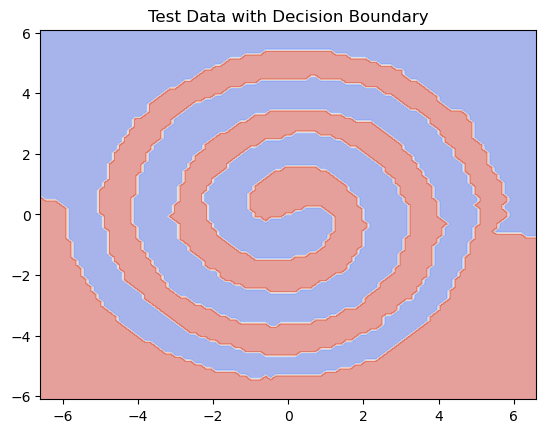
\includegraphics[width=0.5\textwidth]{Question1Images/1AFinalFFNNOutput.png}
  \caption{Average Decision Boundary over 10 folds}
  \label{fig:FirstFFNNDecision}
\end{figure}

\subsection{Part b}

Text for Part b.

\subsection{Part c}

Text for Part c.

\section{Question 2}

\subsection{Part a}

Text for Part a.

\subsection{Part b}

Text for Part b.

\section{Conclusion}

Conclusion text.

\pagebreak
\appendix
\section{Appendix}

\subsection{Question 1}

\counterwithin{table}{chapter}
\begin{table}[ht]
  \centering
  \caption{Results of 2 Layer Architectures}
  \begin{tabular}{c c c c c}
    \toprule
    Epochs \quad & Hidden Neurons \quad & Learning Rate \quad & Average Test Loss \quad & Average Test Accuracy \\
    \midrule
    100 & 8  & 0.01 & 0.84 & 0.38 \\
    300 & 16  & 0.02 & 1.61 & 0.37 \\
    1000 & 16  & 0.02 & 4.91 & 0.42 \\
    \bottomrule
  \end{tabular}
  \label{tab:1A2LayerResults}
\end{table}

\counterwithin{figure}{chapter}
\begin{figure}[!htb]
  \centering
  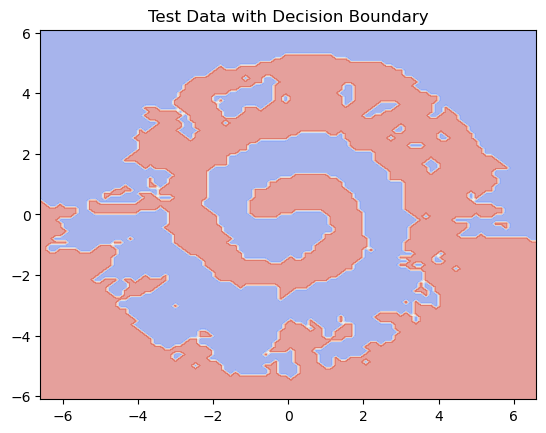
\includegraphics[width=0.5\textwidth]{Question1Images/firstFFNNOutput.png}
  \caption{Average Decision Boundary over 10 folds}
  \label{fig:FirstFFNNDecision}
\end{figure}

\begin{table}[ht]
  \centering
  \caption{Final Model Architecture}
  \begin{tabular}{c c c}
    \toprule
    Epochs \quad & Hidden Neurons \quad & Learning Rate \\
    \midrule
    1000 & 64  & 0.01 \\
    \bottomrule
  \end{tabular}
  \label{tab:1AFinalModelArchitecture}
\end{table}

%
%\begin{table}[ht]
%  \centering
%  \caption{Results of FAKE FAKE}
%  \begin{tabular}{c c c}
%    \toprule
%    Learning Rate & Loss & Accuracy \\
%    \midrule
%    0.01 & 0.103 & 0.963 \\
%    0.001 & 0.076 & 0.972 \\
%    0.0001 & 0.066 & 0.978 \\
%    \bottomrule
%  \end{tabular}
%  \label{tab:exp2}
%\end{table}




%\begin{figure}[ht]
%\centering
%\includegraphics[width=0.5\textwidth]{loss.png}
%\caption{Training and validation loss over 100 epochs}
%\label{fig:loss}
%\end{figure}

Figures and tables that were placed into the appendix.

\end{document}
